\section{\bf Introduction}
% no \IEEEPARstart
In early February 2012 the director of the Philadelphia Science Festival asked the Drexel Autonomous Systems Lab (DASL)\footnote{Drexel Autonomous Systems Lab: http://dasl.mem.drexel.edu}\label{foot:dasl} if they could have their full-size humanoid Jaemi Hubo throw the ceremonial first pitch at the second annual \textit{Science Night at the Ballpark}.  
On April 28th, 2012 Hubo successfully threw the first pitch at the Philadelphia Phillies vs. Chicago Cubs game in front, see Fig.~\ref{fig:hubo-throw}.
There were 45,196 fans at the game and thousands more were watching it on telivision acording to USA Today.

\begin{figure}[t]
  \centering
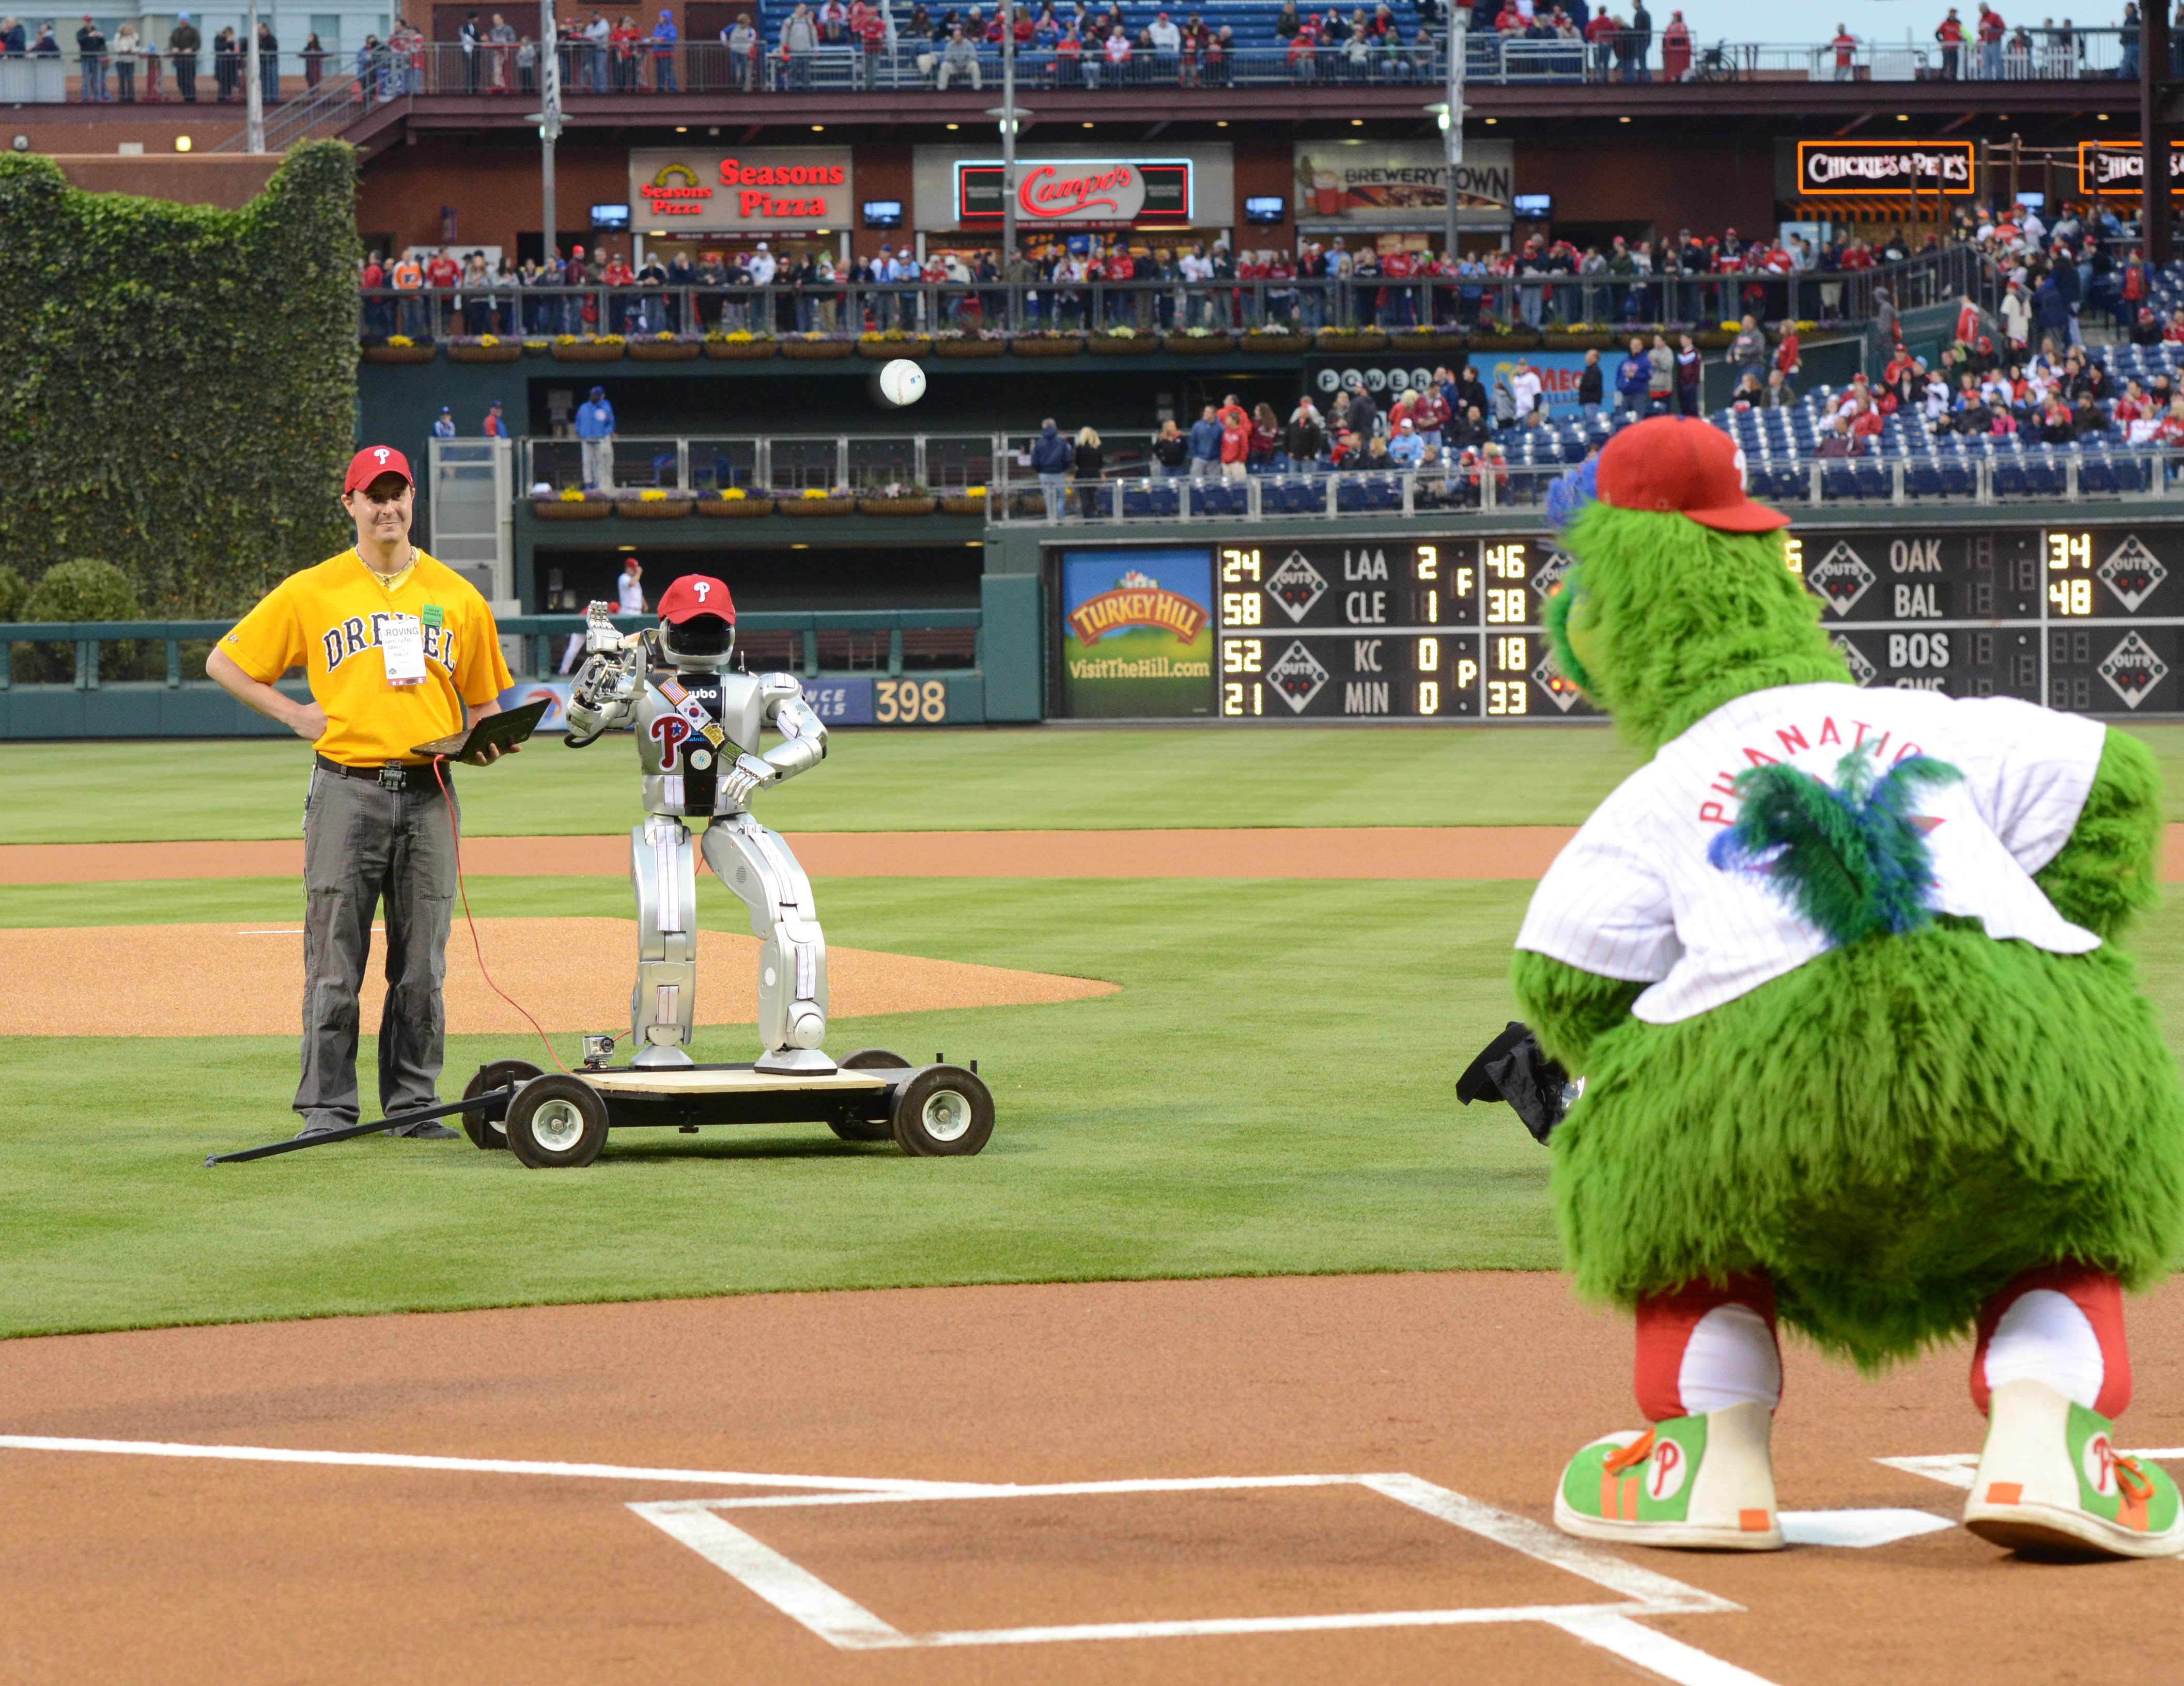
\includegraphics[width=1.0\columnwidth]{./pix/hubo-pitch.png}
  \caption{Hubo successfully throwing the first pitch at the second annual Philadelphia Science Festival event Science Night at the Ball Park on April 28th, 2012.  The game was between the Philadelphia Phillies and the Chicago Cubs and played at the Major League Baseball stadium Citizens Bank Park.  The Phillies won 5-2.  Video of the pitch can be found at http://danlofaro.com/urai2012/\#pitch}
  \label{fig:hubo-throw}
\end{figure}


%The PhillieBot\footnote{PhillieBot Video: http://youtu.be/ShId-vZ-ZEY} made by the GRASP Lab at the University of Pennsylvania was the robot that threw the first pitch at the first annual Philadelphia Science Festival \textit{Science Night at the Ballpark} in 2011.  

Hubo was the first full-size humanoid to throw the inaugural pitch at a Major League Baseball game.  
This task poses challenges in the area of fully-body locomotion, coordination and stabilization that must be addressed.
This paper describes how the latter was done via the analyses/tests of three different approaches and the resulting final design.
Section~\ref{sec:background} gives a brief introduction to work already done in the field as well as states the requirements for the pitch.
Section~\ref{sec:methodology} describes the three different methods tested with a focus on the human-robot kinematic mapping approach.  
The fully automated approach that uses the sparse reachable map (SRM)\cite{dlofaro-srm} and key-frame trajectory generation methods are also explored.
Section~\ref{sec:comparison} compares the tests and analyses of each of the methods.
Section~\ref{sec:finalDesign} describes the finial design in detail and the modifications needed to make the robot's pitch reliable.
Section~\ref{sec:conclusion} gives final thoughts and possible improvements for future years.


%% remember robust and to say that you learned from upenns mistakes etc.